\documentclass{beamer}
\usefonttheme[onlymath]{serif}
\usepackage[english]{babel}							%For internationalization
\usepackage[utf8]{inputenc}							%For character encoding
\usepackage{amsmath}								%For mathematical typesetting
\usepackage{amssymb}								%For mathematical typesetting
\usepackage{graphicx}								%For handling graphics

\newcommand{\be}{\begin{equation}}
\newcommand{\bea}{\begin{equation*}}
\newcommand{\ben}[1]{\begin{equation}\label{#1}}
\newcommand{\ee}{\end{equation}}
\newcommand{\eea}{\end{equation*}}
\newcommand{\aq}{\overset{\sim}{q}}

\title
{An Introduction to Discontinuous Galerkin Methods}
\subtitle{Module 2: A Simple 1D DG Solver}
\author[Bevan] % (optional, for multiple authors)
{J.~Bevan}
\institute[UMass Lowell]
{
  Department of Mechanical Engineering, Grad Student\\
  University of Massachusetts at Lowell
}
\date[Fall 2014]
{}
\subject{Discontinuous Galerkin}

\begin{document}
\frame{\titlepage}
\frame{\frametitle{Module 2: A Simple 1D DG Solver}\tableofcontents}

%NEW SECTION
\section{Linear Solution Approximation} 
\subsection{Definition}
\frame{\frametitle{\textbf{\secname}: \subsecname}
\begin{itemize}
\item The exact sol'n $q(x)$ is not usually obtainable, the best we can do is an approximate sol'n $\aq(x)$
\item We can think of the approximate solution belonging to some finite vector space $\aq \in V_h$, this vector space must have a set of basis vectors $\psi$ such that
\be \aq(x) = \sum_{i=0}^M a_i \psi_i(x) \ee
\item We will choose $V_h$ in this simple example to be the space of all polynomials of order 1 and less: $\mathbb{P}^M, M=1$
\item Because $M=1$, we must have two basis functions. We shall choose two ramp functions, let's see what they look like...
\end{itemize}
}

\subsection{Bases and Resultant Approximation} 
\frame{\frametitle{\subsecname}
\begin{itemize}
\item Basis funs (blue) $\psi_0(x) = 1-x$ and (red) is $\psi_1(x)=x$. Resultant approximation is linear: $\aq(x) = a_0(1-x) + a_1(x)$
\end{itemize}
\begin{figure}
\centering
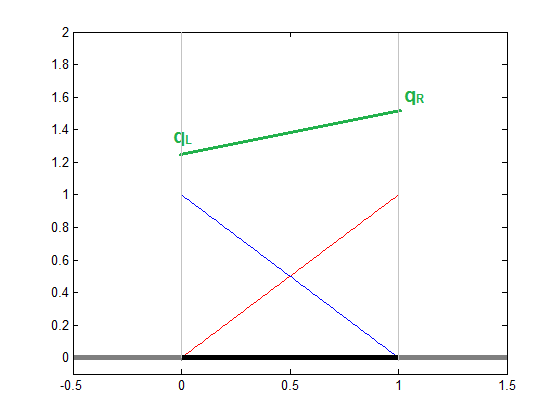
\includegraphics[width=4in]{linearBasis.PNG}
\end{figure}
}

%NEW SECTION
\section{Test Function Choice (Galerkin)} 
\frame{\frametitle{\textbf{\secname}}
\begin{itemize}
\item We have now defined our approximation space, but what about the weighting function in the weak form: $\phi$?
\item We will discuss this in greater detail, but as in a FEM, DG chooses the space of weighting functions to be the same as the approximation space, $\phi \in V_h$
\item This means our weighting functions are ramp functions as well $\phi_0(x) = \psi_0(x), \phi_1(x) = \psi_1(x)$
\item In order to solve for the approximation, our weak form sol'n must be satisfied for \textit{each} weighting function.
\end{itemize}
}

%NEW SECTION
\section{Upwind Flux} 
\frame{\frametitle{\textbf{\secname}}
\begin{itemize}
\item If our flow is incompressible and the global domain is 1D, we must have a constant flow with velocity $c$ everywhere.
\item Let's assume that $c>1$, the numerical flux is then $c\aq^-$ at all boundaries 
\item Note that there are two distinct numerical fluxes for element $k$, on the left it is $cq^-(x_L)$ and the right $cq^-(x_R)$ , where $q^-(x_L)$ doesn't necessarily equal $q^-(x_R)$
\end{itemize}
\begin{figure}
\centering
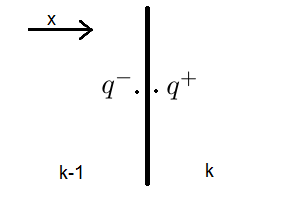
\includegraphics[width=1.5in]{qBoundary.PNG}
\end{figure}
}

%NEW SECTION
\section{Mass Matrix} 
\frame{\frametitle{\textbf{\secname}}
\be \int_k\! \frac{\partial \aq}{\partial t} \,\phi_j \,dx +
	[f(\aq)\phi_j] \Big\rvert_{x_L}^{x_{R}} -
	\int_k\! f(\aq) \,\frac{d\phi_j}{dx} \,dx = 0 \quad for\, all\, j\leq N\ee
\begin{itemize}
\item From convention for dynamic systems the left integral in the weak form is called the \textit{mass matrix}
\item We now have explicit formula for $\aq$ and $\phi$, substituting
\be \int_k\! \frac{\partial \aq}{\partial t} \,\phi_n \,dx = \sum_{i=0}^M \frac{d a_i(t)}{dt} \int_k \psi_i(x) \phi_j(x) \ee
\end{itemize}
}
\frame{\frametitle{\secname}
\bea \int_k\! \frac{\partial \aq}{\partial t} \,\phi_n \,dx = \sum_{i=0}^M \frac{d a_i(t)}{dt} \int_k \psi_i(x) \phi_j(x)\,dx \eea
\begin{itemize}
\item Let's substitute in our expressions for approximation and the first weighting basis and analytically integrate
\be \int_k \psi_i(x) \phi_0(x)\,dx=\qquad\qquad\qquad\qquad \Big|_0^1\ee
\item Do this for each weighting basis to get 2x2 matrix: $\mathbf{M}_{j,i}$
\item If the time derivative of each of the approximation coefficients is a vector $\mathbf{a'}$ then
\be \sum_{i=0}^M \frac{d a_i(t)}{dt} \int_k \psi_i(x) \phi_j(x) \,dx = \mathbf{M}\,\mathbf{a'}  \ee
\end{itemize}
}


%NEW SECTION
\section{Stiffness Matrix} 
\frame{\frametitle{\textbf{\secname}}
\bea \int_k\! \frac{\partial q}{\partial t} \,\phi \,dx +
	[f(q)\phi] \Big\rvert_{x_L}^{x_{R}} -
	\int_k\! f(q) \,\frac{d\phi}{dx} \,dx = 0 \eea
\begin{itemize}
\item Similar to mass matrix, substitute our approximation and bases into the third term.
\be \int_k\! f(q) \,\frac{d\phi}{dx} \,dx = \sum_{i=0}^M c a_i(t) \int_k \psi_i(x) \phi'_j(x) \,dx \ee
\item The integral for all weighting bases combine to form the stiffness matrix $\mathbf{K}$, we can analytically integrate for this simple case
\end{itemize}
}

\frame{\frametitle{\secname}
\begin{itemize}
\item Similar to the mass matrix, we have a vector of our element approximation coefficients $\mathbf{a}$, such that
\be \sum_{i=0}^M c a_i(t) \int_k \psi_i(x) \phi'_j(x) \,dx =  \mathbf{K}\,\mathbf{a}\ee
\item Let's substitute in our expressions for approximation and the first weighting basis and analytically integrate
\be \int_k \psi_i(x) \phi'_0(x)\,dx=\qquad\qquad\qquad\qquad \Big|_0^1\ee
\end{itemize}
}


%NEW SECTION
\section{Putting it all Together} 
\frame{\frametitle{\textbf{\secname}}
\begin{itemize}
\item Just need to calculate the numerical flux vector now.
\be [\hat{f}(q)\phi] \Big\rvert_{x_L}^{x_{R}} = cq_k(x_R)\phi_j(x_R)- cq_{k-1}(x_R)\phi_j(x_L)\ee
\item $\phi_j$ will be zero sometimes, depending on $j$
\item So what do we get?
\item $\mathbf{\hat{f}}=$
\end{itemize}
}

%NEW SECTION
\section{Semi-discrete system} 
\frame{\frametitle{\textbf{\secname}}
\begin{itemize}
\item We can now express the semi-discrete system compactly in matrix/vector form
\be \mathbf{M}\,\mathbf{a}'  + \mathbf{\hat{f}} - c\mathbf{K}\,\mathbf{a} =0 \ee
\item For each time step we have $\mathbf{a}$, starting with $\mathbf{a}_0$ from ICs
\item We'd like to calculate the time rate of change of our coefficients to use in our time discretization, so solve for $\mathbf{a}'$
\be \,\mathbf{a}'  = \left[c\mathbf{K}\,\mathbf{a} -\mathbf{\hat{f}}\right]\mathbf{M}^{-1} \ee
\end{itemize}
}

%NEW SECTION
\section{Time Discretization: Forward Euler} 
\frame{\frametitle{\textbf{\secname}}
\begin{itemize}
\item Now we need to complete the method by discretizing in time the semi-discrete system
\item Let's use a Forward Euler approach; very simple explicit ODE solver
\be \mathbf{a}_{t+1} = \mathbf{a}_t+ \mathbf{a}'_t \Delta t\ee
\item We can overwrite our previous timestep's coefficients with the new ones to save memory
\item We may want to periodically save $\mathbf{a}$ for plotting
\item We must choose $\Delta t$ carefully, can you predict why?
\end{itemize}
}

%NEW SECTION
\section{Investigation- h-Convergence} 
\frame{\frametitle{\textbf{\secname}}
\begin{itemize}
\item What do we expect for h-convergence?
\item How coarse can our elements be and still get a "good-enough" answer?
\item What effect does the shape/smoothness of the solution have on convergence?
\end{itemize}
}

%NEW SECTION
\section{Investigation- t-Convergence} 
\frame{\frametitle{\textbf{\secname}}
\begin{itemize}
\item How big can we make $\Delta t$?
\item Do we expect periodic solutions to stay steady over time?
\item How do h and t convergence relate?
\end{itemize}
}

%NEW SECTION
\section{Investigation- Stability (CFL)} 
\frame{\frametitle{\textbf{\secname}}
\begin{itemize}
\item As was seen, too large of a timestep lead to issues, why?
\item What happens if a parcel of quantity moves fast enough to skip elements between timesteps?
\item We need to ensure
\be CFL = \frac{c \Delta t}{\Delta x} \leq C_{max}=1 \ee
for explicit methods. Implicit methods relax this restriction to permit higher values.
\end{itemize}
}

\end{document}